\chapter{Fase iniziale}
In questo capitolo verrà esposta la fase iniziale del progetto: come è nata l'idea e quali sono stati i primi passaggi per gettare una solida base di un'applicazione che potesse risultare valida.

\section{Idea}
Alla base del workshop vi era sostanzialmente una gara tra team di programmatori con lo scopo di premiare l'applicazione migliore secondo parametri quali la scalabilità e utilità per il grande pubblico.
Studiando varie idee per il nostro progetto, abbiamo cercato di trovare un punto comune tra tutti i membri. Il principale punto di congiunzione tra noi era il fatto di vivere a pieno la vita da universitari con relativi problemi e difficoltà. Per questo abbiamo provato ad elaborare una soluzione ad almeno uno dei vari problemi che ci affliggevano e, di conseguenza, affliggevano gli altri studenti di tutte le univiversità.
Primo tra tutti, a rendere faticosa la vita studentesca, è il ‘viaggio’ giornaliero per raggiungere le sedi: ogni mattina uno studente si alza e sà che dovrà correre più veloce del tram per non perderlo e arrivare in ritardo a lezione. La maggior parte degli studenti, infatti, ogni giorno intraprende una vera e propria odissea per raggiungere le università a causa del traffico, dei ritardi dei mezzi pubblici e di tutte le scomodità che un pendolare può conoscere.
Una volta individuato il problema, ci siamo messi a lavoro per trovare una soluzione basandoci sulle idee proposte dai competitors e adattandole poi alla figura dello studente medio: da qui il nostro motto “For students. By students”.
Sono stati presi in considerazione diversi approcci al problema fino a giungere alla conclusione che quello del ride pooling fosse il più appropriato, perché in grado di unire il taglio dei costi e il fattore social.
A differenza del più famoso car sharing in cui l'utente di fatto noleggia un' auto, il ride pooling consiste nella condivisione di un passaggio e dei relativi costi come benzina e/o parcheggio.
Il possesso di un mezzo privato, per quanto conveniente, comporta molteplici costi, dal carburante al mantenimento, passando per il parcheggio e l’assicurazione; la condivisione invece permette di ripartire una parte di questi tra più persone; portando all’ammortamento dei costi intrinsechi del tragitto e alla riduzione del numero delle macchine in circolazione. Tutto ciò attraverso la messa in contatto di studenti, così da favorire l’incontro tra le diverse realtà universitarie e magari fare nuove amicizie.

\section{Convalida dell'idea}
Al fine di concretizzare il nostro lavoro ed essere sicuri che il progetto avesse un effettivo valore per il suo bacino di utenti, avevamo bisogno di un riscontro con il futuro pubblico dell’applicazione. Per questo è stato sottoposto un sondaggio ad un gran numero di studenti delle principali università di Roma.
Il sondaggio non doveva essere complesso per evitare di avere risultati falsati dalle risposte randomiche di eventuali studenti frettolosi nel rispondere e sostanzialmente anche perchè i concetti cardine da rilevare erano pochi.
Oltre il 75\% ( Figura \ref{fig:graph1} ) dei partecipanti al sondaggio ha risposto positivamente alla domanda “Utilizzeresti il servizio MoveMate?”.
Alla domanda “Come useresti il servizio?” quasi il 50\% ( Figura \ref{fig:graph2} ) era interessato al fattore social della nostra applicazione così da poter conoscere altre persone.
A tal fine abbiamo aggiunto la possibilità di "condividere" anche il viaggio con mezzi pubblici.
L’interesse da parte degli studenti ci ha dato coraggio nel continuare il nostro progetto.

\begin{figure}[!h]
\begin{minipage}{\linewidth}
  \centering
    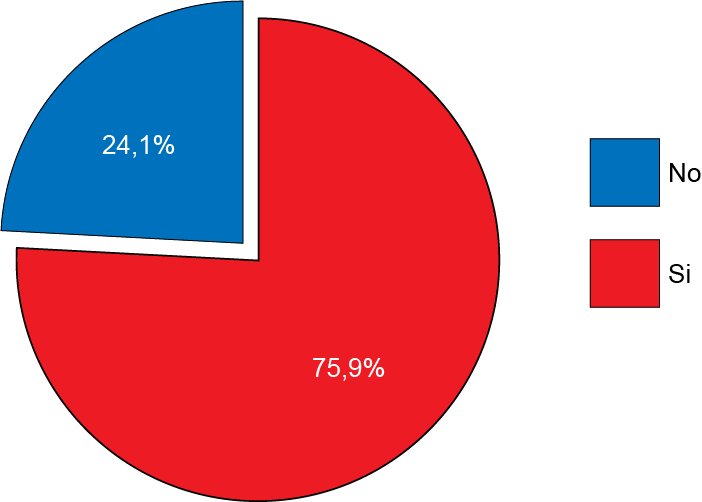
\includegraphics[width=0.6\textwidth]{graph1}
  \caption{Snapshot risultati 1}
  \label{fig:graph1}
\vspace{1cm}
  \centering
    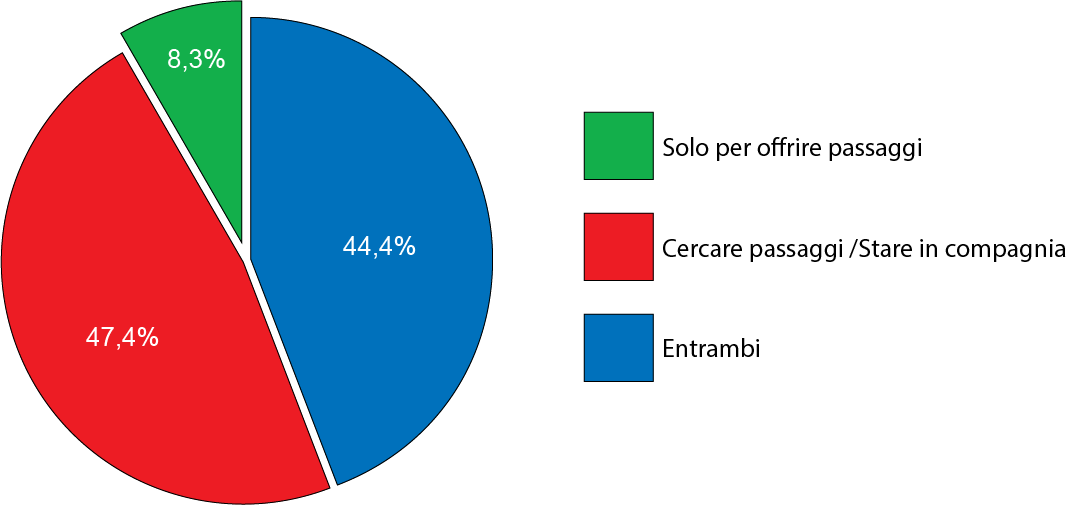
\includegraphics[width=0.9\textwidth]{graph2}
  \caption{Snapshot risultati 2}
  \label{fig:graph2}
\end{minipage}
\end{figure}

\FloatBarrier


